\renewcommand{\theequation}{\theenumi}

\begin{enumerate}[label=\arabic*.,ref=\thesubsection.\theenumi]
\item In $\triangle ABC$,
\begin{equation}
\label{eq:linea}
\vec{A}=\myvec{1\\2}
\end{equation}
%
and the equations of the medians through $\vec{B}$ and $\vec{C}$
are respectively
\begin{align}
\label{eq:line_medb}
\myvec{1 & 1}\vec{x}&=5
\\
\myvec{1 & 0}\vec{x}&=4
\label{eq:line_medc}
\end{align}
%
Find the area of $\triangle ABC$.
\\
\solution The centroid $\vec{O}$ is the solution of \eqref{eq:line_medb},\eqref{eq:line_medc} and is obtained 
as the solution
of the matrix equation
\begin{align}
\myvec{1 & 1 \\1 & 0}\vec{x}&=\myvec{5 \\ 4}
\label{eq:line_matrix}
\end{align}
%
which can be solved using the augmented matrix as follows.
\begin{align}
\myvec{1 & 1 & 5\\1 & 0 & 4} \leftrightarrow \myvec{1 & 1 & 5\\0 & 1 & 1}\leftrightarrow  \myvec{1 & 0 & 4\\0 & 
1 & 1}
\end{align}
Thus,
\begin{equation}
\label{eq:lineo}
\vec{O}=\myvec{4\\1}
\end{equation}
% 
Let  $AD$ be the median through $\vec{A}$. Then,
\begin{align}
\frac{\vec{A}+\vec{B}+\vec{C}}{3}&= \vec{O}
\\
\implies \vec{B}+\vec{C}= 3\vec{O}-\vec{A} &= \myvec{11 \\ 1}
\label{eq:line_b+c}
\\
\implies \myvec{1 & 1}\vec{B}+\myvec{1 & 1}\vec{C}&=  \myvec{1 & 1}\myvec{11 \\ 1}
\label{eq:line_ctemp}
\end{align}
%
From \eqref{eq:line_medc} and \eqref{eq:line_ctemp},
\begin{align}
 \myvec{1 & 1}\vec{B} &= 5 
\\
\implies 5+\myvec{1 & 1}\vec{C}&=  12
\\
\implies \myvec{1 & 1}\vec{C}&=  7
\label{eq:line_ctemp2}
\end{align}
From \eqref{eq:line_ctemp2} and \eqref{eq:line_medc}, $\vec{C}$ can be obtained by solving 
\begin{align}
\myvec{1 & 1 \\1 & 0}\vec{C}&=\myvec{7 \\ 4}
\label{eq:line_cmatrix}
\end{align}
using the augmented matrix as
\begin{align}
\myvec{1 & 1 & 7\\1 & 0 & 4} &\leftrightarrow \myvec{1 & 1 & 7\\0 & 1 & 3}\leftrightarrow \myvec{1 & 0 & 4\\0 & 
1 & 3}
\\
\implies \vec{C}&=\myvec{4\\3}
\end{align}
%
From \eqref{eq:line_b+c},
\begin{align}
\vec{B}&=\myvec{11\\1}-\myvec{4\\3}
=\myvec{7\\-2}
\end{align}
%
Thus,
\begin{align}
\frac{1}{2}
\begin{vmatrix}
\vec{A} & \vec{B} &\vec{C}
\\
1 & 1 & 1
\end{vmatrix}
=
\frac{1}{2}
\begin{vmatrix}
1 & 7 & 4\\2 & -2 & 3 \\ 1 & 1 & 1
\end{vmatrix} = 9
\end{align}
\item Summarize all the above computations through a Python script and plot $\triangle ABC$.
\\
\solution
\begin{lstlisting}
https://github.com/gadepall/school/raw/master/linalg/2D/manual/codes/triang.py
\end{lstlisting}
\begin{figure}
\centering
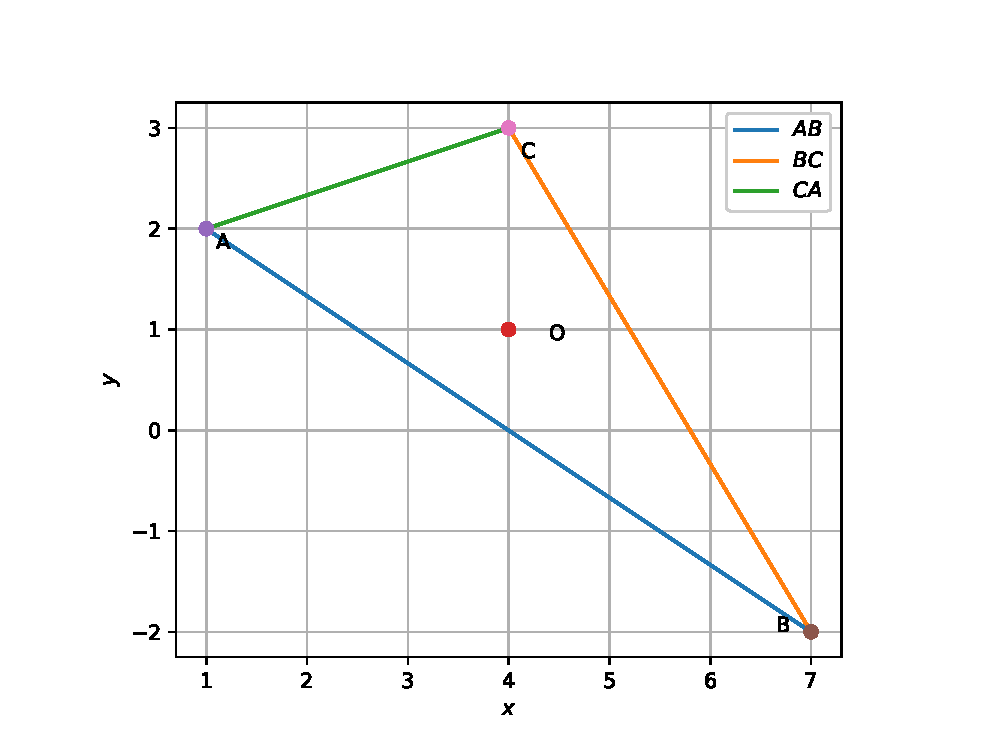
\includegraphics[width=\columnwidth]{./line/figs/triangle.eps}
\caption{}
\label{fig:triangle}
\end{figure}
\item
Find the coordinates of $\vec{D}, \vec{E}$ and $\vec{F}$ of the mid points of $AB, BC$ and $CA$ respectively 
for  $\Delta ABC$. 
\item
Find the equations of $AD,BE$ and $CF$. 
%
\item
\label{prob:median}
Find the point of intersection of $AD$ and $CF$.
\item
Verify that $\vec{O}$ is the point of intersection of $BE,CF$ as 
well as
\item
Graphically show that the medians of $\Delta ABC$ meet at the centroid.
\item
In $\Delta ABC$,  Let $\vec{P}$ be a point on $BC$ such that $AP \perp BC$.  Then $AP$ is defined to be 
an {\em altitude} of $\Delta ABC$.

\item
\label{prob:alt_eq}
Find the equation of $AP$.
\\
\solution The normal vector of $AP$ is $\vec{B} - \vec{C}$. From 
\eqref{eq:line_norm}, the equation of $AP$ is
\begin{align}
\label{eq:alt_ap}
\brak{\vec{B} - \vec{C}}^T\brak{\vec{x} - \vec{A}}&= 0
\\
\implies \myvec{-3&4}\vec{x} = -\myvec{-3&4}\myvec{2\\2} &= -2
\end{align}

%\lstinputlisting{./codes/alt_eq.py}
%
\item Find the equation of the altitude $BQ$.
\\
\solution The desired equation is 
\begin{align}
\label{eq:alt_bq}
\brak{\vec{C} - \vec{A}}^T\brak{\vec{x} - \vec{B}}&= 0
\\
\implies \myvec{6&1}\vec{x} = \myvec{6&1}\myvec{1\\3} &= 9
\end{align}
\item Find the equation of the altitude $CR$.
%
\item Find the point of intersection of $AP$ and $BQ$.
\solution \eqref{eq:alt_ap} and \eqref{eq:alt_bq} can be stacked together into the matrix equation
\begin{align}
\label{eq:alt_mat}
 \myvec{-3&4 \\ 6&1}\vec{x} = \myvec{-2\\9}
\end{align}
The following code computes the point of intersection.
\begin{lstlisting}
https://raw.githubusercontent.com/gadepall/school/master/linalg/2D/python_2d/codes/orthocentre.py
\end{lstlisting}

\item Find the point of intersection of  and $BQ$ and $CR$. Comment.
\item Find $\vec{P}$
%
\\
\solution The following code finds the required points.
\begin{lstlisting}
https://raw.githubusercontent.com/gadepall/school/master/linalg/2D/python_2d/codes/alt_foot.py
\end{lstlisting}
\item Find $\vec{Q}$ and $\vec{R}$.
\item Draw $AP, BQ$ and $CR$ and verify that they meet at a point 
$\vec{H}$.  
\\
\solution The following code plots the altitudes in Fig. \ref{fig:alt_triangle}
\begin{lstlisting}
https://raw.githubusercontent.com/gadepall/school/master/linalg/2D/python_2d/codes/alt_draw.py
\end{lstlisting}
%\begin{figure}
%\centering
%\includegraphics[width=\columnwidth]{./figs/alt_triangle.eps}
%\caption{}
%\label{fig:alt_triangle}
%\end{figure}
\end{enumerate}

